\documentclass[letterpaper,10pt,twoside]{book}
\usepackage[spanish]{babel}
\usepackage[utf8]{inputenc}
\usepackage{graphicx}
\usepackage{tikz}
\usepackage{wallpaper} 
\usepackage{color}

\usepackage{imakeidx}
\usepackage[backend=bibtex,style=numeric,sorting=ynt]{biblatex}
\usepackage{url}
\addbibresource{bibliografia.bib}
\makeindex


\newcommand{\receta}[1]{
\chapter*{#1}
\addcontentsline{toc}{chapter}{#1}
}

\newenvironment{ingredientes}{
\section*{Ingredientes}
\begin{itemize}
\setlength{\itemsep}{0pt}
\setlength{\parsep}{0pt}
\setlength{\parskip}{0pt}}
{\end{itemize}}

\newcommand{\preparacion}{
\section*{Preparación}
}

\newcommand*\rfrac[2]{{}^{#1}\!/_{#2}}

\begin{document}
\title{Recetas de Familia}
\author{Andrés Hurtado López}
\date{2017}
\pagenumbering{gobble}
\begin{titlepage}
	\addtolength{\wpXoffset}{-12cm}
	\addtolength{\wpYoffset}{-3cm}
	\ThisCenterWallPaper{2.5}{fotos/portada.jpg}

	\definecolor[named]{color01}{rgb}{0.92,0.92,0.33}

	\begin{tikzpicture}[remember picture,overlay]
		\node [rectangle, rounded corners, fill={RGB:red,150;green,150;blue,150}, opacity=0.50, anchor=south west, minimum width=21.6cm, minimum height=18cm] (box) at (-2.6cm,-21cm) (box){};

		\node[text centered, anchor=north, color01, text width=21.6cm, yshift=-1cm,font=\Huge\bfseries\fontsize{80}{80}\selectfont ] at (box.north){ RECETAS DE FAMILIA }; 

		\node[text centered, anchor=south, white, yshift=1.5cm, text width=20cm, font=\bfseries\LARGE] at (box.south)(name){\textbf{Andrés Hurtado López}};
				\node[text centered, anchor=south, white, yshift=1.5cm, text width=20cm, font=\bfseries\LARGE] at (name.south){\textbf{Primera Edición}};


	\end{tikzpicture}
	\clearpage

  	\begin{center}
    	\large
    	ANDRÉS HURTADO LÓPEZ \\
    	\vspace*{3cm}
    	\Huge{Recetas de Familia} \\
    	\vspace*{5cm}
    	\normalsize
    	%Editor\\
    	%Liliana Herrera Ramirez\\
    	%\vspace*{1cm}    
    	%Diseño Gráfico\\
    	%Ana Maria Hurtado\\
    	%\vspace*{1cm}
    	%Fotografia \\
    	%Juan Pablo Hurtado\\
    	%\vspace*{1cm}
    	Dirección Técnica \\
    	Luz Stella López\\
    	\vspace*{6.5cm}
    	Andrés Hurtado\\
    	2017\\
  	\end{center}
\end{titlepage}
\pagenumbering{roman}
\frontmatter
ficha tecnica libro
\chapter{Agradecimientos}
A todas mis tias y mis tios gracias por su inifita paciencia aguantando toda mi intensidad durante la recolección de las recetas. \\

A mi Mamá por ternerme, criarme, aguantarme y mamare todo éste proceso de creación de éste libro.
\chapter{Dedicatoria}
A mis abuelitas y tia: No se imaginan lo que disfruté y lo que me falta por disfrutar, esta vá por ustedes.
\chapter{Prefacio}
Mi característica barriga no es un caso desafortunado del destino, tengo un alto grado de certeza que mi tradición familiar culinaria jugó un papel trascendental en su proceso evolutivo en línea curva. No tengo arrepentimientos en mi vida al respecto, los manjares de mis predecesores es algo que realmente he disfrutado y llevo en mi corazón en todos los años que llevo sobre la faz de la tierra. Creo que disfrutaré estos placeres hasta el final de mi existencia.\\

Fué un arduo trabajo lograr recopilar y convertir todas las recetas a un formato normalizado tanto en nombres de ingredientes como unidades de medida dada la diversidad cultural de personas aportaron piezas a este compendio. La idea general es poder brindar un conjunto de recetas deliciosas que sus medidas y nombres de ingredientes se preserven y sean reproducibles a través de los años, para que medidas regionales o temporales tales como \emph{``5 centavos''} o \emph{``una pucha''} no se conviertan en un obstáculo. En general todas las recetas se procuraron convertir en medidas de masa en sistema internacional de medidas (SI) en donde fue posible.\\

Por curioso que parezca, la combinación de gustos de todos mis parientes dá para un muy variado ramillete de platos que ván desde lo simple y mundano pero a la vez reconfortante para el alma, hasta los platos más exóticos y asombrosos. Éste documento busca mantener vivos en el tiempo algunos de esos platos maravillosos que reconfortaron mi alma durante el sagrado momento donde todos compartimos en la mesa.


\tableofcontents
\mainmatter
\part{Comida de Sal}
\makeatletter\@openrightfalse
\receta{Spaguetti con Verduras y Especias}

Rinde para 3 personas.\\

\begin{ingredientes}
\item 250g Spaguetti
\item 400g Pimentón
\item 520g Calabazin amarillo
\item 430g Berengena
\item 16g Jalapeños
\item 411g Tomates maduros hervidos (en lata)
\item Aceite de Oliva
\item Sal
\item Paprika al gusto
\item Pimienta negra al gusto
\item 1 Cucharada de Azucar
\item 10g Ajo
\item Agua
\end{ingredientes}
\preparacion
Se parten la berenjenas en tajadas redondas, el calabazin en tajadas redondas, el pimentón en julianas. La berenjena se pone a remojar en salmuera hecha con el agua y la sal hasta que el agua se torne levemente color café.\\

Se sofrie la berenjena en una sartén en aceite de oliva de forma que las tajadas queden doradas. Usando el mismo aceite se sofrie el pimentón y el calabazin.\\

En una olla se pone a hervir agua y despues se pone a cocinar la pasta. Para el tiempo de cocción de la pasta ver el tiempo recomendado en el empaque.\\

En una olla aparte se pone aceite, paprika, pimienta, ajo y jalapeño finamente picados  hasta que ajo dore. A esta mezcla se le incorpora los tomates hermidos picados y una cucharada de azucar dejando reducir 10 minutos.\\

Se saca la pasta cocinada y se incorpora con el resto de los ingredientes.

\receta{Spaguetti con Carne}

Rinde para X personas.

\begin{ingredientes}
\item 1kg Ingrediente
\end{ingredientes}
\preparacion


\receta{Carne con Verduras y Azucar}
Esta receta salió de una de las revistas de mi abuelita, esta carne tiene algo especial que no se describir con palabras, a pesar de que el titulo suena algo horroroso por combinar carne con azúcar, puedo asegurar que su sabor es muy diferente a su titulo ya que de azúcar solo tiene una cucharada.

Esta receta es para 8 porciones de 230 g. Es excelente para se combinada con arroz blanco al vapor.

Valor nutricional por cada 100g de Carne con verduras :
\begin{itemize}
\item Energia: 153 kcal
\item Carbohidratos: 7.3g
\item Grasas: 8.2g
\item Proteínas: 12.7g
\end{itemize}

Rinde para 5 personas.

\begin{ingredientes}
\item 13g Azucar
\item 320g Pimenton Rojo y/o verde
\item 250g Cebolla partida solo en 4
\item 500g Champiñones laminados
\item 68g Fecula de maiz (Maizena)
\item 64g Salsa Soya (soja o como le digan)
\item 120g Aceite vegetal (yo usé canola)
\item 1000g Carne de Res mas o menos magra (Yo usé lomo)
\item 2 Tazas de agua
\item 2 Taza de arroz blanco
\end{ingredientes}
\preparacion
Por aparte en en una olla se pone a hervir el arroz como se hace usualmente hervido. Se pican en tiras los pimentones, se parten las cebollas en 4 separando las laminas de las cebollas. Estos ponen a saltear en un wok con 61g de aceite hasta que ablanden.\\

Se incorporan los champiñones laminados y de deja cocinar con el resto de las verduras. Una vez queden todas las verduras salteadas se sacan aparte del wok en una olla mas grande. Con la salsa soya, la fecula de maiz y el agua se hace una mezcla en un recipiente aparte.\\

En el wok se pone el aceite restante con la carne y se pone la carne a sofreir agregando lentamente la mezcla de salsa soya hecha anteriormente hasta lograr que la carne quede en su punto y la salsa espese, revisando constantemente el gusto de sal de la carne para adobarle en caso que haga falta.\\

Una vez lista la carne se incorporta con el resto de las verduras en la olla mas grande, es este punto se debe generar en a olla una salsa espesa de color café. A esta mezcla se le agrega el azucar y se deja reducir.\\

Se sirven porciones de 230g de carne con verdura y 200g de arroz.
\receta{Costillas Pegajosas de Kansas City}

Rinde para X personas.


\begin{ingredientes}
\item 2 Medias canales de costilla de cerdo que con el exeso de membrana y grasa removidos
\item Para adobar las costillas:
\begin{itemize}
\item 3 Cucharadas de paprika
\item 2 Cucharadas de azucar morena
\item 1 Cucharada de pimienta negra molida
\item 1 Cucharada de sal
\item 1/4 de cucharadita de pimienta cayena
\end{itemize}
\item Para la salsa complementaria:
\begin{itemize}
\item 2 Cucharaditas de Aceite de cocina
\item 1 Cebolla cabezona picada
\item 4 tasas de caldo de pollo
\item 1 taza de cerveza de raiz (ponymalta)
\item 1 taza de vinagre de cidra o vinagre de manzana.
\item 1 taza de jarabe de maiz obscuro
\item 1/2 taza de melaza de caña
\item 1/2 taza de pasta de tomate
\item 1/2 taza de ketchup
\item 2 cucharadas de mostaza cafe o mostaza antigua
\item 1 cucharada de salsa de tabasco
\item 1/2 cucharadita de polvo de ajo
\item 1/2 cucharadita de escencia de olor a ahumado. (opcional)
\end{itemize}
\end{ingredientes}
\preparacion

\emph{Para la Salsa}\\


\emph{Para las Costillas}\\

Tomar todos los ingredientes para adobar la costilla y mezclarlos en un recipiente aparte hasta que la mezcla quede uniforme.\\

Secar las costillas de la sangre que aun tenga impregnadas y a continuacion “sobar” las costillas con la preparacion de adobo mezclada de paso anterior hasta que queden totalmente impregnada por toda su superfecie asegurandose que el total de la mezcla quede sobre la superficie de las costillas, en caso de que no se vean como en las siguientes fotos aumentar las cantidades de la mezcla para adobo en iguales proporciones.\\

Precalentar el horno hasta alcanzar los $150^{\circ}C$ ($300^{\circ}F$) e introducir las costillas adobadas inicialmente por 45 min. Despues de debe dejar mas tiempo vijilando el color de la superficie de las costillas hasta asegurase que obtengan un color caramelo pero que no se queme la superficie. Una buena tecnica para poder hacer esto es disminur la temperatura del horno a $100^{\circ}C$($212^{\circ}F$) hasta lograr el color, lo cual lo puede hacer un poco demorado. Con esto las costillas quedan listas para ser servidas acompañadas de la salsa.\\

\receta{Lomito Alcaparrado}
\index{lomito alcaparrado}

Rinde para 6 personas.

\begin{ingredientes}
\item  Preparación Lomo
\begin{itemize}
\item 1.5 kg de Lomo Viche
\item 4 Dientes de Ajo grandes
\item 1 Cucharada de Salsa Inglesa
\item Sal
\item Pimienta
\item Mantequilla para freír el lomo
\end{itemize}
\item Salsa:
\begin{itemize}
\item 30 g Mantequilla
\item 75 g Harina de trigo
\item 1 Cubo de caldo de carne
\item 2 Tazas de Agua
\item 200 g Alcaparras 
\item 150 g uvas pasas
\item Sal
\item Pimienta
\end{itemize}

\end{ingredientes}
\preparacion
Con 1 dia de anticipación, procesar finamente el ajo hasta obtener una pasta para adobar el lomo acompañado con la salsa inglesa, sal y pimienta.\\

En el momento de la preparación derretir la mantequilla en una sartén y freir el lomo por ambos lados.\\

En la misma sartén donde se doró la carne, colocar los 30 g de Mantequilla y dejarla derretir,  incorporar poco a poco la harina y el cuo de caldo. Verter el agua y revolver continuamente.Agregar las alcaparras y las uvas pasas, salpimentar si es necesario. Dejar hervir hasta que las mezcla espese.\\

Colocar en una refractaria el lomo y bañarlo con esta salsa. Llevar al horno precalentado a $350^\circ$F ($177^\circ$C) durante $\rfrac{1}{2}$ hora.

\begin{center}
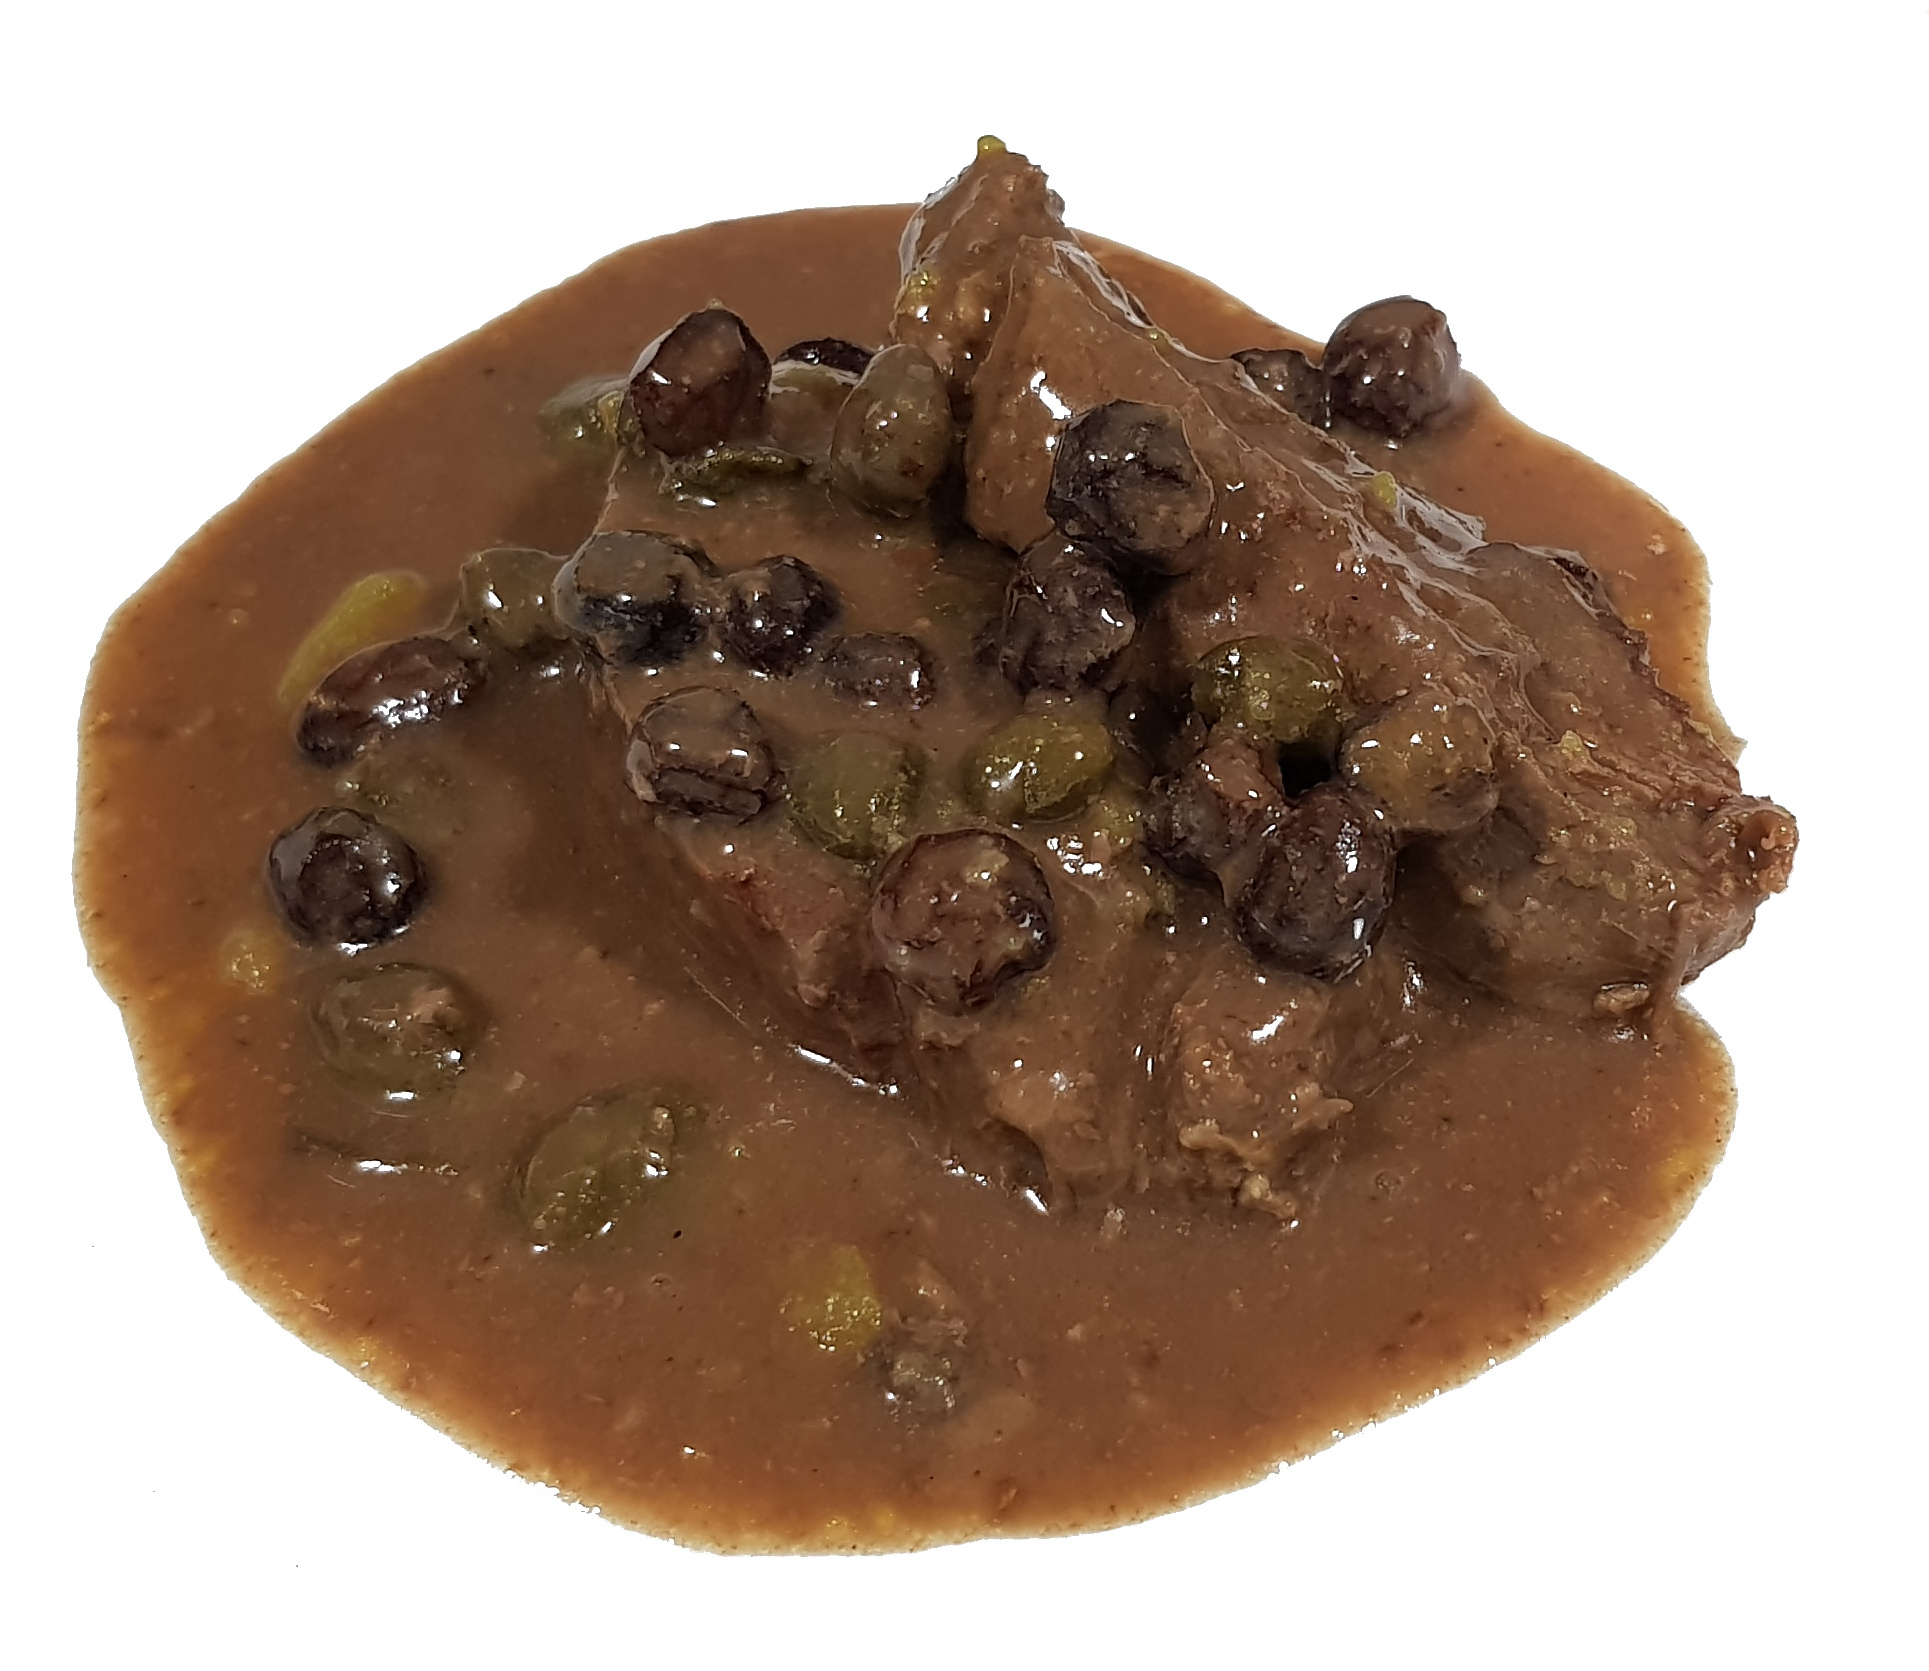
\includegraphics[width=0.8\textwidth]{fotos/lomito_alcaparrado.jpg}
\end{center}
\receta{Marranitas}

Rinde 18 Unidades.

\begin{ingredientes}
\item 9 Plátanos Maduros
\item 1.5 kg Tocino
\item 1 L Aceite 
\item Agua
\item Bolsa plástica
\end{ingredientes}
\preparacion

Se cortan el tocino en cubos pequeños y se fritan para obtener chicharrones. Por aparte se pelan los plátanos y se cortan a la mitad de forma que salgan 2 troncos por plátano los cuales se fríen hasta que queden ligeramente dorados. .\\

Los troncos se pisan hasta obtener un masa que permita armar arepitas de plátano que se se les pone abundante agua para que le masa sea maleable.\\

A las arepitas mojadas se le ponen cubitos de chicharrón encima y con la masa se encierran los chicharrones formando bolitas. Para ayudar al proceso de cerrado se una una bolsa plástica para ayudar a mantener la forma de bola sin que se desbarate la masa.\\

Las bolitas se ponen a freir nuevamente hasta que queden doradas y se retiran rápidamente del aceite mientras este bien caliente para que no absorban mas grasa.\\
\clearpage
\vspace*{5cm}
\begin{center}
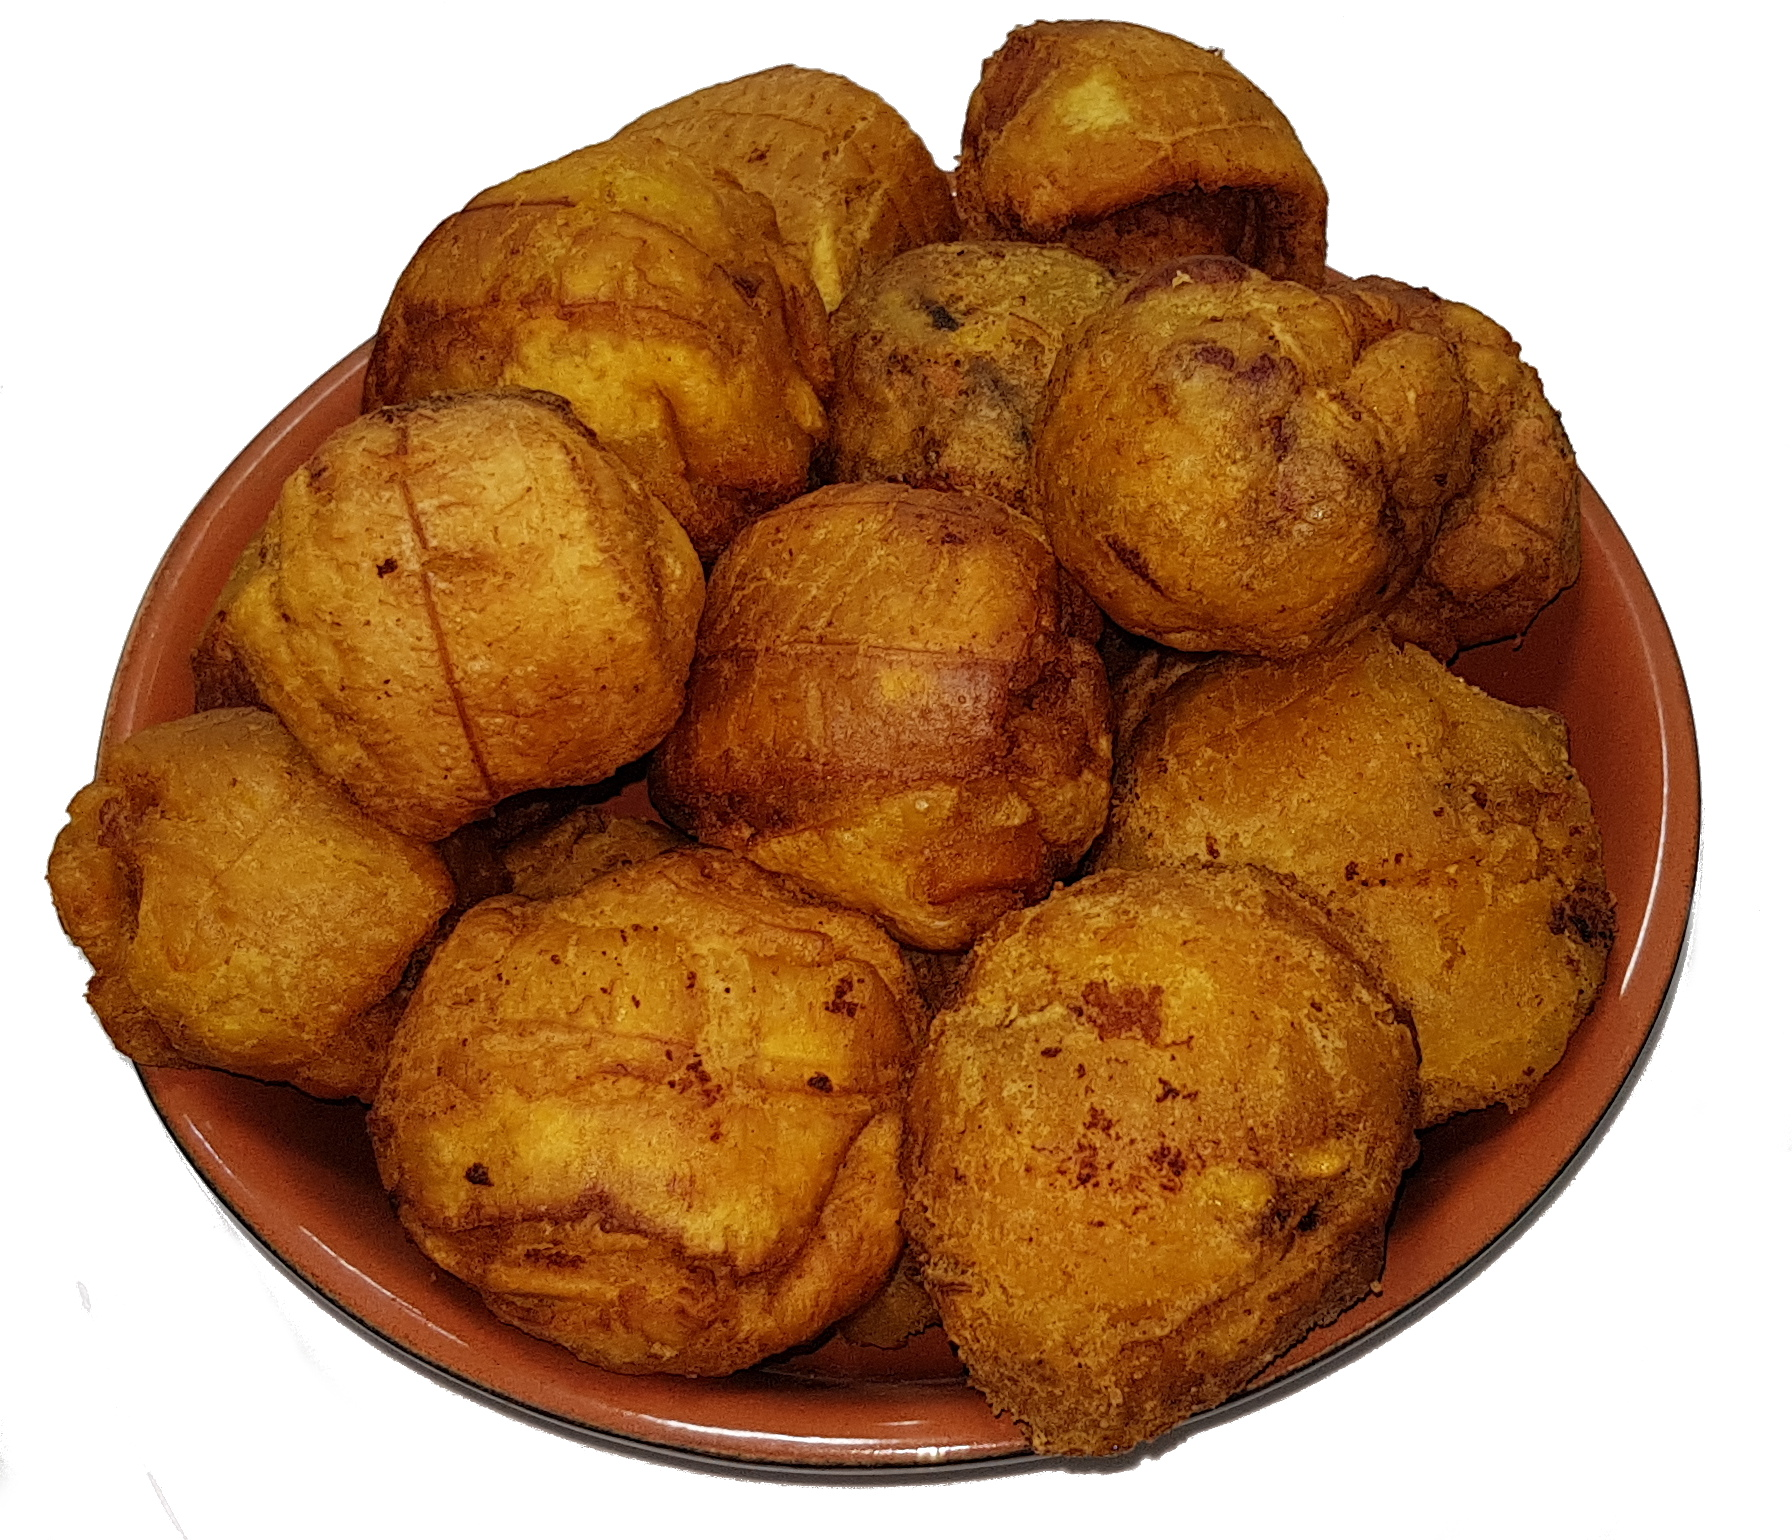
\includegraphics[width=0.8\textwidth]{fotos/marranitas}
\end{center}
\receta{Molde de Berenjena, Tomate y Queso Mozzarela}

Rinde para X personas.


\section*{Ingredientes}
\begin{itemize}
\setlength{\itemsep}{0pt}
\setlength{\parsep}{0pt} \setlength{\parskip}{0pt}
\item 1kg Ingrediente
\end{itemize}
\section*{Preparación}



\receta{Molde Atún}

Rinde para X personas.\\

\begin{ingredientes}
\item Atun en aceite
\item Papas
\item Cebolla de Huevo
\item Pimentón
\item Pimiemta
\item Mayonesa
\item Huevos
\item Queso Parmesano
\end{ingredientes}
\preparacion

Se pelan y cocinan las papas en agua. Se pone a hervir por aparte tiras de pimentón y cebolla para desaguarlas. Tambíen se ponen a hervir huevos hasta que queden duros y se parten en rodajas.Las papas cocinadas se vuelven puré y se sasonan con pimienta y por aparte se escurre el atún y se le agrega mayonesa.\\

En un molde refractario plano se aplica una capa moderada de puré de papa, encima una capa de atún con mayonesa, encima una capa de cebolla con algunas tiras de pimenton intercaladas, encima una capa de rodajaa de huevos y se termina con otra capa de puré de papa. Sobre la última capa de puré se pone queso parmesano.\\

El molde se pone al horno a $170^{\circ}C$ hasta que que el queso gratine.

\receta{Lomo Viche En Salsa de Champiñones}
Esta es una receta que preparo mi tia Martha Muñoz para el fin de año, que cosa tan rica, sirve para cualquier ocación especial:
\begin{ingredientes}
\item 4 lb de Lomo biche (solomo) en tajadas de 250gr
\item Mostaza
\item Salsa Inglesa
\item Sal
\item Aceite
\item Mantequilla
\item 1 Sobre mezcla para crema de champiñones
\item 1 Plato ondo Agua
\item 1 cubo magui
\item 1 copa de vino blanco
\item Sal
\item Champiñones tajados crudos
\item Pimienta de moler
\item 1 copa de vino blanco
\end{ingredientes}
\preparacion
Se prepara una mezcla la mostaza y la salsa inglesa adobada con sal al gusto.\\

Con la salsa preparada se impregnan las tajas de carne de lomo crudas de forma abundante que queden cubiertas sus dos caras.\\

En la estufa, en un perol ondo grande se le vierte aceite y mantequilla dejando que se derrita la mantequilla y acance una temperatura para freir la carne.\\

Las tajadas impregnadas de salsa se pasan por el perol de manera que frian cada una de sus caras hasta que queden selladas y no destilen sangre. El proceso anterior se puede hacer con la cantidad de tajadas maxima que pueda caber en el perol donde las carnes queden totalmente extendidas. Las carnes que han terminado el proceso se pueden poner aparte en un plato.\\

Para la base de la salsa se roma el aceite restante del proceso de sellado de la carne se deja calentar de forma que la sangre y salsa sean reducidos lo maximo posible intentando obtener un liquido mas o menos translucido.\\

En  un plato sopero con agua se agrega un sobre de mezcla de crema de champiñones, un cubo magui y se sazona con sal al gusto homogenizando la mezcla la cual se vierte en el aceite traslucido de proceso de sellado de la carne dejando hervir toda la mezcla para que reduzca y espese. Dependiendo de la consistencia deseada de la salsa se puede dejar mas tiempo al fuego agregando mas mezcla de crema de champiñones para aumentarla la viscozidad o agregar mas agua para disminuirla.\\

Al obtener la salsa deseada se agregan los champiños tajados en un pero abarte y se saltean un mantequilla, sazonandolos con pimiento negra molida. El resultado se incorpora a la salsa de champiñones controlando la viscocidad de la misma como se decribio en el paso anterior.\\

Finalmente se incorpora la carne sellada y una copa de vino que estaba por aparte dejando hervir mas tiempo toda la mezcla para que la carne absorba la salsa dejando hervir al gusto sin que se seque la carne. En caso de que la carne y la salsa se sequen mucho se puede agregar agua.


\receta{Lomo Saltado}

Rinde para X personas.\\

\begin{ingredientes}
\item $\rfrac{1}{2}$ kg Lomo de res
\item 2 Tomates picados en tiras
\item 2 Cebollas picada en tiras
\item 1 Ají amarillo picado en tiras
\item 3 Cucharadas de Vinagre
\item 3 Cucharadas de Agua
\item 50g Culantro picado
\item 1 Cucharada de ajo molido
\item $\rfrac{1}{2}$ Taza de Aceite
\item 8 Papas pelada y picadas
\item 3 Cucharadas Salsa de Soya
\item Sal
\item Pimienta
\end{ingredientes}
\preparacion
Picar el lomo de res en cubitos y condimentarlos con sal, pimienta y ajo. Calentar la mitad del aceite en un cartén y freir los lomitos de res hasta dejarlos dorados y reservarlos.\\

Transladar y caletar el resto del aceite en la misma sartén, donde se dora la cebolla, el tomate, el ají con un poco de sal movmiendolo constantemente para que no se pegue. Añadir vinagre, el agua y la salsa de soya. Cuando rompa el hervor incluir los lomitos de res y las hojas de culantro. Combinar y mezclar bien dejando freir todo durante 3 minutos.\\

El resultado se le agregan las papas fritas las cuales se mezcla y se sirven acompañadas de arroz blanco.
\receta{Cazuela de Tortilla Mexicana Frita}
Rinde para 7 Personas.\\
\begin{ingredientes}
\item 330g cebolla de huevo o blanca
\item 938g tomate chonto maduro
\item 663g chorizo de cerdo
\item 880g frijoles chiles zenu (2 tarros)
\item 410g queso mozzarela cremoso molido
\item Aguacate
\item Limones
\item Cilantro
\item Vinagre
\item Sal
\end{ingredientes}
\preparacion
Se corta el tomate en cuartos y se licúa con sal al gusto. Por aparte se cortan en rodajas los chorizos y se corta la cebolla en julianas. Paso seguido se ralla el queso mozzarela.\\

Se sofríe cebolla en julianas hasta obtener punto de caramelo. Se agrega el chorizo y el tomate licuado. A fuego alto se deja reducir toda la mezcla; El punto adecuado de reducción, se observa en la siguiente fotografìa. Este proceso toma próximamente 30 minutos.\\

Por aparte se macera aguacate a discreción,con la cebolla procesada finamente al gusto, adicionar vinagre, sal y cilantro para finalmente se obtener un guacamole cremoso.\\

Los frijoles enlatado se calientan en horno microhondas y finalmente el emplatado se arma con una cama inferior de tortillas fritas de maíz levemente machacadas sobre el plato agregando el resto de ingredientes uno a uno, encima del otro como se puede ver en las fotos a continuacion. Finalmente se revuelve todo el contenido en el interior de plato.
\receta{Paella de mariscos}
La receta es producto de la viajadera y tenaz estudio culinario de mi cansado tio Guillermo.\\

Rinde para 14 personas.


\section*{Ingredientes}
\subsection*{Para El Caldo}
\begin{itemize}
\setlength{\itemsep}{0pt}
\setlength{\parsep}{0pt} \setlength{\parskip}{0pt}
\item 1 Cabezas de pescado grande (corbina, mero, pargo rojo)
\item 1 rama de cebolla larga
\item Comino
\item Pimienta
\item Sal
\item Triguisar
\item 15 tazas de Agua
\end{itemize}
\subsection*{Para El Arroz}
\begin{itemize}
\setlength{\itemsep}{0pt}
\setlength{\parsep}{0pt} \setlength{\parskip}{0pt}
\item 5 tazas de arroz parbolizado o arroz bomba espanol
\item Aceite de oliva
\item 800gr Cebolla cabezona
\item 600gr Tomate chonto
\item 3 pimentones en lajas
\item 1 sazonador de paella
\item 30 Gambas grandes (3 lb)
\item 1kg Anillos de calamar
\item 500 gr Mix de mariscos
\item 1kg pulpo
\item 1kg camarones
\item 1lb mejillones
\item 1lb almejas
\item Manteca de cerdo
\item Ajo
\item Vino blanco
\end{itemize}
\section*{Preparación}
Poner todos los ingredientes para el caldo en una olla a llama completa hasta que la carne suelte la sustancia, que no se pase de 40min.\\

Por aparte, se le retiran los intestinos a los langostinos, secandolos despues para que el agua no salpique cuando se pongan a sofreir. Es muy importante que todos los mariscos queden secos; Mi tio dice que para las Gambas no se debe hacer el procedimiento de lavado porque le “quita el sabor” según los españoles.\\

Se debe utilizar para la cocción una paellera con su respectiva estufa, ya que se necesita que tenga muy buena area para evaporar durante la coccion del arroz. Sobre esta paellera se sofrien las gambas en aceite de oliva hasta que estas dejen la grasa de color pardo y se sacan de la paellera dejando la grasa producto del sofrito como base para sofreir las verduras.\\

Con la grasa producto de las gambas se sofrie: el ajo, cebolla, pimenton, tomate, cuando todos esten sofritos se pasa a agregar el calamar y el pulpo, adiconando sal, pimienta y el sazonador. Finalmente se ponen las almejas fijandose que se abran.

Se procede a poner el arroz en la paellera para sofreirlo sobre todo el mix anteriormente preparado, la idea es que este tome los aromas de todos los mariscos. Como dato curioso los españoles tienen la superticion de que el arroz debe ser regado en forma de cruz, supongo que será para “santificar” el plato.\\

Cuando se vea un color pardo sobre el arroz se agrega el caldo de pescado, este servirá como un liquido sustituto del agua donde hervira el arroz para que el grano abra. En la mitad del proceso de coccion del arroz agregamos mejillones enterrandolos en el arroz en disposicion de anillos. Cuando se halla evaporado todo el caldo, se tapa con papel aluminio y se espera aproximadamente 20 minutos.
\receta{Lasagna Betty}
Esta receta la llama así porque desde que tengo uso de razón la conozco como la lasagna que hacia mi abuelita. Un gran problema de ésta receta es que en ningún lado había copia escrita, todo estaba en la cabeza de mis tías y mi abuela, razón por lo cual en una tarde de domingo, pedimos dirección técnica a mi mama (cosa que sabe hacer bastante bien) y logramos sacar la siguiente aproximación de la receta original. \\

Rinde para 30 personas.

\begin{ingredientes}
\item 3 kg Pechugas hervidas sin hueso
\item 3 kg Pierna de cerdo
\item 500 g Tocineta
\item 2 Cubitos de Caldo de gallina
\item 3 kg Tomates en trozos en latados
\item 800 g Pasta de tomate
\item 1 Cebolla de huevo
\item 4 Dientes de ajo
\item 1.5 kg Pasta de lasagna precocida
\item 1.5 kg Queso Holandes
\item 1.5 kg Queso parmesano
\item 345 g Crema de leche
\item Laurel Seco
\item Tomillo
\item Sal
\item Especias Italianas (Italian Seasoning)
\item 1 Manojo de Perejil picado.
\end{ingredientes}
\preparacion
Pone a cocinar el pollo y la carne de cerdo en una olla pitadora, se le hecha los cubitos de caldo de gallina, unas hojas de laurel y sal. Se pone a cocinar hasta que ablande. Cuando todo ablanda, se saca a un plato a enfriar, se deshebran las dos carnes. El caldo en que se cocinaron las carnes se reserva para mas adelante.\\

Se coloca en una sarten la tocineta a sofreir, se saca aparte en un plato dejando la grasa en la sartén. Se pica la cebolla y el ajo finamente y con la grasa de la tocineta se sofríen, si se necesita mas grasa se le adiciona aceite.\\

Se procesa los trozos de tomate para que queden en puré y se le agregan a la mezcla  de la cebolla en conjunto con la pasta de tomate, tomillo y laurel, dejándola en el fuego hasta que la mezcla tome un color rojo obscuro. Se le agregan el pollo y la carne de cerdo y se revuelve bien y poco a poco.\\

Se se le va agregando el caldo en que se cocino la carne hasta darle una consistencia de salsa, ya que de por si es muy seca y pastosa mezcla. Se deja a fuego lento, a medio tapar, para que todos los sabores se incorporen a la mezcla vigilando que no se seque, caso en el cual se le agrega el caldo.\\

Se le debe estar probando constantemente el sabor para verificar si requiere adiconarle sal a la mezcla. Para darle un toque final a la salsa se desmorona la tocineta, se le hecha un la crema de leche y el perejil picado.\\

En un molde refractario se pone una capa de salsa, encima una capa de pasta de lasagna remojada previamente en agua tibia y encima una capa de queso holandés y queso parmesano. Este proceso se repite varias veces armando capas hasta llegar al borde del molde. Lugar en el cual se debe acabar con una capa de queso,  es cubierta finamente con salsa y queso parmesano para gratinar la cubierta superior.\\

Todo se mete en horno precalentado a $350^\circ$F ($177^\circ$C) dejando hervir, que el queso parmesano quede derretido y el interior de la lasgna caliente.\\






\receta{Arroz con Espinacas}

Rinde para X personas.


\section*{Ingredientes}
\begin{itemize}
\setlength{\itemsep}{0pt}
\setlength{\parsep}{0pt} \setlength{\parskip}{0pt}
\item 1kg Ingrediente
\end{itemize}
\section*{Preparaci�n}



\receta{Fríjoles}

Rinde para X personas.


\section*{Ingredientes}
\begin{itemize}
\setlength{\itemsep}{0pt}
\setlength{\parsep}{0pt} \setlength{\parskip}{0pt}
\item 1kg Ingrediente
\end{itemize}
\section*{Preparación}



\receta{Lentejas}

Rinde para X personas.


\section*{Ingredientes}
\begin{itemize}
\setlength{\itemsep}{0pt}
\setlength{\parsep}{0pt} \setlength{\parskip}{0pt}
\item 1kg Ingrediente
\end{itemize}
\section*{Preparaci�n}



%\receta{Sancocho de U�a}

Rinde para X personas.


\section*{Ingredientes}
\begin{itemize}
\setlength{\itemsep}{0pt}
\setlength{\parsep}{0pt} \setlength{\parskip}{0pt}
\item 1kg Ingrediente
\end{itemize}
\section*{Preparaci�n}



%\receta{Sopa Platano Frito}

Rinde para X personas.


\section*{Ingredientes}
\begin{itemize}
\setlength{\itemsep}{0pt}
\setlength{\parsep}{0pt} \setlength{\parskip}{0pt}
\item 1kg Ingrediente
\end{itemize}
\section*{Preparación}



%\receta{Sopa Arróz}

Rinde para X personas.


\section*{Ingredientes}
\begin{itemize}
\setlength{\itemsep}{0pt}
\setlength{\parsep}{0pt} \setlength{\parskip}{0pt}
\item 1kg Ingrediente
\end{itemize}
\section*{Preparación}



%\receta{Sancocho}

Rinde para X personas.


\section*{Ingredientes}
\begin{itemize}
\setlength{\itemsep}{0pt}
\setlength{\parsep}{0pt} \setlength{\parskip}{0pt}
\item 1kg Ingrediente
\end{itemize}
\section*{Preparación}



%\receta{Sopa Arracacha}

Rinde para X personas.


\section*{Ingredientes}
\begin{itemize}
\setlength{\itemsep}{0pt}
\setlength{\parsep}{0pt} \setlength{\parskip}{0pt}
\item 1kg Ingrediente
\end{itemize}
\section*{Preparación}



\receta{Hogo (Guiso)}

Rinde para X personas.


\begin{ingredientes}
\item Tomate
\item Cebolla
\item Triquisar
\item Comino
\item Aceite
\item Pimienta
\item Sal
\end{ingredientes}
\preparacion
En una sartén se sofrie el tomate y luego se hecha la cebolla con aceite hasta que cubra los ingredientes dejandolo llegar a punto de ebullicion. Finalmente se adoba con triguisar, pimienta, comino y sal al gusto.



%\input{contenido/ensalada_papa}
%\receta{Empanadas}

Rinde para X personas.


\section*{Ingredientes}
\begin{itemize}
\setlength{\itemsep}{0pt}
\setlength{\parsep}{0pt} \setlength{\parskip}{0pt}
\item 1kg Ingrediente
\end{itemize}
\section*{Preparaci�n}



\receta{Achuchas (Pepinos rellenos)}

Rinde para X personas.


\section*{Ingredientes}
\begin{itemize}
\setlength{\itemsep}{0pt}
\setlength{\parsep}{0pt} \setlength{\parskip}{0pt}
\item 1kg Ingrediente
\end{itemize}
\section*{Preparación}



\receta{Albondigas}

Rinde para X personas.

\begin{ingredientes}
\item Carne Molida
\item Huevo
\item Salsa Negra
\item Miga de pan
\item Comino
\item Pimienta negra
\item Sal
\item Cebolla
\item Tomate
\item Ajo
\item Perejil
\item Cilantro
\item Aceite
\item Cubo caldo de gallina
\item Tajada Pan
\end{ingredientes}
\preparacion
A la carne molida se le mezcla comino, pimienta negra, sal, salsa negra y se amasa hasta obtener una mezcla homogenea. Esta mezcla se cubre con miga de pan con huevo para que se adhiera sazonandola .\\

Se arman albondigas de la mezcla anterior  y se sofrien en aceite. En la licuadora se pone cebolla, tomate, perejil, cilantro, caldo de gallina, la tajada de pan y agua hasta obtener una salsa que se pone a reducir en una olla a fuego lento.\\

Se pelan las papas y se parten a la mitad para luego ponen a hervir en agua. Estas se agregan en la olla de la salsa con las albondigas sofritas, dejando cocinar un poco más.
\receta{Berenjenas}

Rinde para X personas.


\section*{Ingredientes}
\begin{itemize}
\setlength{\itemsep}{0pt}
\setlength{\parsep}{0pt} \setlength{\parskip}{0pt}
\item 1kg Ingrediente
\end{itemize}
\section*{Preparación}



%\receta{Rollo de Carne}

Rinde para X personas.


\section*{Ingredientes}
\begin{itemize}
\setlength{\itemsep}{0pt}
\setlength{\parsep}{0pt} \setlength{\parskip}{0pt}
\item 1kg Ingrediente
\end{itemize}
\section*{Preparación}



%\receta{Lengua de Res}

Rinde para X personas.


\begin{ingredientes}
\item 1kg Ingrediente
\end{ingredientes}
\preparacion
Se cocna la lengua y se pela. Se vuelve a poner a cocinar con sal. Cuando la lengue este blandita se taja.

Por aparte se pone a freír ajo, cebolla cabezona picada en mantequilla, al ratico se le pone orégano, laurel, tomillo y se deja sazonar un rato. Luego se incorporan 2 tazas de caldo maggi, se deja cocinar na ratico, se baja, se cuela y se le echa salsa de tomate.

Para la salsa se ponen 2 cucharadas grandes de mantequilla derretida se le ponen 2 cucharadas de harina de trigo. Cuando este bien incorporado se le echa 1 taza de leche. Esto se deja hervir un ratico y se le pone el caldo y 1 copa de vino. Esta salsa se revuelve con la lengua y se deja sazonar y si queda clara la salsa se le pone mas harina y por ultimo se le echan las arvejas o champiñones frito en mantequilla


\receta{Crepes de Atún}

Rinde para X personas.


\begin{ingredientes}
\item 5 Latas de atún
\item 6 Ramas de Apio
\item 1 Lata de crema de leche
\item Mayonesa
\item Margarina
\item Harina
\item Sal
\item Pimienta
\item Leche
\item Queso Parmesano
\end{ingredientes}
\preparacion
\emph{Para el relleno:} Se mezcla el atún escurrido, el apio picado, la crema de leche y mayonesa.\\

\emph{Para la Salsa:} En un olla se pone margarina con harina se lentamente se va adicionando leche, revolviendo constantemente y se adoba con sal y pimienta. Cuando la salsa esté espesa se le agrega crema de leche y queso parmesano.\\

\emph{Para los Crepes:}

\emph{Ensamble:} Se rellenan los crepes, se cierran y en una refractaria se colocan bañandolos encima con la salsa dejandolos que doren.

%\receta{Crema de Cebolla}

Rinde para X personas.


\section*{Ingredientes}
\begin{itemize}
\setlength{\itemsep}{0pt}
\setlength{\parsep}{0pt} \setlength{\parskip}{0pt}
\item 1kg Ingrediente
\end{itemize}
\section*{Preparaci�n}



\receta{Soufflé de Atún}

Rinde para X personas.


\begin{ingredientes}
\item 2 latas de atún
\item 2 pimentones
\item 2 cebollas cabezonas
\item 3 Sobres de gelatina sin sabor
\item $\rfrac{1}{2}$ frasco de mayonesa
\item 3 Cucharadas de salsa de tomate
\item 6 tajas de pan trituradas
\item perejil crespo
\item $\rfrac{3}{4}$ tasa de agua
\end{ingredientes}

Picar finamente la cebolla
Picar el perejil
Hervir $\rfrac{1}{2}$ tasa de agua.
Remojar la gelatina en $\rfrac{1}{4}$ de tasa de agua fría 

\preparacion



%\receta{Lomo de Cerdo Acaramelado}

Rinde para X personas.


\section*{Ingredientes}
\begin{itemize}
\setlength{\itemsep}{0pt}
\setlength{\parsep}{0pt} \setlength{\parskip}{0pt}
\item 1kg Ingrediente
\end{itemize}
\section*{Preparación}



\receta{Sopa de Mondongo}

%Rinde para X personas.

\begin{ingredientes}
\item 1 Kg de mondongo
\item 1 Kg de carne de cerdo
\item 1 Kg de costilla de cerdo
\item 150g Arroz ($\rfrac{1}{2}$ taza)
\item 1 Yuca grande
\item 6 Papas Grandes
\item 500g de Alberjas
\item 3 Chorizos
\item Hogo
\item Ajo
\item Azafran
\item Cominos
\item Pimienta
\item Cebolla
\item Tomate
\item Limón
\item Color
\item Hogo (Ver receta pagina \pageref{hogo})
\end{ingredientes}
\preparacion
En una olla express se coloca el callo ò mondongo con agua y se deja cocinar hasta que este quede tierno. A continuación utilizando la misma agua resultante de le cocción se procede igualmente a cocinar la carne de cerdo hasta que esta también ablande. La carne y el mondongo se ponen aparte y en el caldo resultante se pone a cocinar el arroz, la papa, yuca y la alverja hasta que la mezcla espese.\\

En una sartèn se fríen los chorizos y se pican en trocitos al igual que el cerdo y el mondongo apartados anteriormente. Todo se pone junto en la olla inicial del caldo y se deja calar con hogo. Al finalizar se le agrega el comino.
%\receta{Coliflor en su Salsa}

Rinde para X personas.


\section*{Ingredientes}
\begin{itemize}
\setlength{\itemsep}{0pt}
\setlength{\parsep}{0pt} \setlength{\parskip}{0pt}
\item 1kg Ingrediente
\end{itemize}
\section*{Preparaci�n}



%\receta{Muchacho en Salsa de Champi�ones}

Rinde para X personas.


\section*{Ingredientes}
\begin{itemize}
\setlength{\itemsep}{0pt}
\setlength{\parsep}{0pt} \setlength{\parskip}{0pt}
\item 1kg Ingrediente
\end{itemize}
\section*{Preparaci�n}



\receta{Salsa de Tomate}
Esta es la salsa que se utiliza para ponerle a los guarguerones, achuchas, muchaho y lengua entre otros.

Rinde para X personas.

\begin{ingredientes}
\item 6 Tomates maduros
\item 1 cebolla cabezona
\item 2 cebollas largas
\item 1 Ramo de perejil
\item 2 rebanadas de pan
\item 4 Ajos
\item Mantequilla
\item Sal
\item Pimienta
\item Agua
\end{ingredientes}
\preparacion
Seponen en un aolla los tomates partidos en cruz, la cebolla partida en cruz, la cebolla larga, el perejil, el pan, y los ajitos cubiendo todos los ingredientes con agua y se deja a fuego alto a reducir.\\

Se deja enviar la mezcla y se pone en la licuadora. El resultado se pone en un olla con mantequilla, sal y pimienta para adobar y se deba a fuego lento para que espese mediante reducción.\\
%\receta{Pur� Zanahoria}

Rinde para X personas.


\section*{Ingredientes}
\begin{itemize}
\setlength{\itemsep}{0pt}
\setlength{\parsep}{0pt} \setlength{\parskip}{0pt}
\item 1kg Ingrediente
\end{itemize}
\section*{Preparaci�n}



\receta{Arroz con Pollo y Almendras}

Rinde para 4 personas.


\begin{ingredientes}
\item 1 Pechuga de Pollo
\item 270g arroz blanco
\item 40g Mantequilla
\item 70g Almendras
\item 1 Tallo de cebolla larga
\item 8g Ajo
\item $\rfrac{1}{4}$ Cucharadita Pimienta Negra
\item $\rfrac{1}{8}$ Cucharadita Canela
\item $\rfrac{1}{2}$ Cubo de caldo de gallina
\item 700ml Agua
\end{ingredientes}
\preparacion
Picar finamente la cebolla larga, el ajo y hacer perforaciones en la pechuga sin quitarle la piel.
Colocar en una olla express el pollo, 30g de mantequilla, la cebolla, el ajo, la pimienta y la canela hasta que haga el primer vapor \\

Paso seguido se saca el pollo de la olla express, complementando al líquido restante en la olla con agua hasta que en la olla hallan $4\;\rfrac{1}{2}$ tasas de agua. A continuación se agrega todo el arroz y la mantequilla restante, dejando hervir hasta que el arroz quede cocido completamente.

En una olla se pone a hervir agua con las almendras. Cuando se obtenga el primer hervor se sacan las almendras del agua y se les quita las cascara cuando todavía están calientes. Paso seguido se ponen en una sartén con aceite o mantequilla y se doran.

Por último, el pollo se desmenuza y se incorpora al arroz en conjunto con las almendras tostadas y se sirve el plato caliente antes de que las nueces se humedezcan.


%\receta{Tabbule}

Rinde para X personas.


\begin{ingredientes}
\item 1kg Ingrediente
\end{ingredientes}
\preparacion



%\receta{Knefe Be Jeben}

Rinde para X personas.


\section*{Ingredientes}
\begin{itemize}
\setlength{\itemsep}{0pt}
\setlength{\parsep}{0pt} \setlength{\parskip}{0pt}
\item 1kg Ingrediente
\end{itemize}
\section*{Preparación}



\receta{Frijoles Chinos}

Rinde para 6 personas.


\begin{ingredientes}
\item 700 g pocillos de fríjol verde 
\item 1 kg pechugas de pollo
\item 170 g Pimentón
\item 90 g Apio
\item 115 g Cebolla larga
\item 70 g Cebolla de huevo
\item 200 g Tomates maduros
\item 30 g Raíces chinas (Brotes de soya)
\item 2 Papas
\item 1 Cubo de caldo de gallina
\item 70 g Aceite vegetal de cocina
\item 2.5 L Agua
\item Sal
\item Pimienta Negra
\item Comino  
\item Tomillo
\item Salsa Soya
\end{ingredientes}
\preparacion


Se pica finamente por separado tomate, cebolla larga, cebolla de huevo, apio, pimentón y se reservan.

En la olla express se pone toda el agua a cocinar con las pechugas de pollo, 40g de cebolla larga picada, sal, pimienta y caldo de gallina. Cuando el pollo este cocinado, se saca el pollo y el agua que queda se reserva. Las pechugas se desmenuzan las pechugas se desmenuzan y se reservan también por aparte. 

Se hace un hogo utilizando: 75g cebolla larga, toda la cebolla de huevo, todo el apio, todo el pimentón, todo el tomate, sal, pimienta negra, mucho comino, tomillo y salsa soya.

Con el agua reservada de la cocción del pollo se ponen a cocinar los fríjoles verdes en la olla express. Cuando los fríjoles se hallan ablandado se le agrega el hogo preparado anteriormente y el pollo desmenuzado. Todo se deja calar por lo menos 10 minutos hasta obtener una consistencia ligeramente espesa y se le agregan la todas las raíces chinas.

Por aparte se ralla la papa y se fríen en tiras, la cuales al momento de servir los fríjoles se sirven encima como adorno.
\receta{Moqueca de Piexe (Moqueca de Pescado)}

Rinde para X personas.

\begin{ingredientes}
\item Cherna
\item Anillos de calamar
\item Langostinos talla 16
\item Cebolla roja
\item Cebolla blanca
\item Pimenton
\item Tomate
\item Perejil
\item Cilantro
\item Ajo
\item Leche de coco
\item Aceite de dende
\item Aceite de oliva
\item Agua
\item Mantequilla
\end{ingredientes}

\preparacion
Se corta en rodajas pimenton, cebolla y tomate. Se deshojan el perejil y el cilantro. Se limpian los langostinos rompiendo la cascara y quitandoles solamente la vena sin quitar la cascara.\\

En una olla grande se pone aceite de oliva y se revienta unos dientes de ajo a fuego medio a sofreir revolviendo hasta que doren. Sobre el ajo dorado se ponen en capas de espesor parejo cebolla roja, cebolla blanca, pimenton, tomate, perejil, cilantro, el pescado y los calamares. Despues se vuelven a repetir las capas de cebolla, pimenton, tomate, perejil y cilantro y se pone una taza de agua dejando a fuego medio con la tapa de la olla puesta. Pasados 15 minutos se destapa la olla para verificar el nivel del agua y agregar los langostinos cubiertos de mantequilla y ajo. Se vuelve a tapar la olla por 10 minutos revisando el nivel del agua y se agrega la leche de coco y el aceite de dende por 5 minutos mas. Si el nivel del agua esta bajo agregar ,as agua y dejarncocinar más. La preparación debe tener la consiatencia de una sopa.
\receta{Frijoles Chiles}

Rinde para 7 personas.

\begin{ingredientes}
\item 500g Frijoles
\item 2 platanos
\item 500g carne molida de cerdo
\item 3 paquetes de Pasta de tomate
\item hogo
\item Cubos caldo de gallina
\end{ingredientes}
\preparacion
Con un dia de anticipación se ponen a remojar los frijoles en agua. Se pica el platano en cuadro muy finos y en una olla a presión en conjunto con los frijoles y agua se cocinan por 1 hora. Paso seguido, se destapa la olla para comprobar que los frijoles ya hallan ablandado; en caso de que no, volver a cocinar a presion por otros 30 min y repetir hasta obtener consistencia blanda. Con la olla a presión destapada, se agrega la carne molida, la pasta de tomate y el hogo. Si al momento de mezclar la preparación está muy sólida, se le agrega mas agua y cubos de caldo de gallina. Dejar reducir hasta que los frijoles calen.

\receta{Habichuelas con Carne}

Rinde para 4 personas. Aporte calorico por peso 1.66 kcal/g

\begin{ingredientes}
\item 500g Habichuelas Picada
\item 500g Carne de res
\item 250g Pasta de tomate
\item 40g Aceite
\item Agua
\item Sal
\item Pimienta Dulce
\item Pimienta Negra
\end{ingredientes}
\preparacion

Hierva en una olla las habichuelas picadas en cuadritos y resérvelas con el agua. Sofría la carne con el aceite, y posteriormente agregue la pasta de tomate. Cuando  la pasta se torne obscura, agregue las habichuelas con el agua para formar salsa, dejando reducir a fuego medio. Finalmente, cuando la consistencia de la salsa sea espesa, se adoba la mezcla con las pimientas y la sal.



\receta{Bisquec a Caballo (Steak \& Eggs)}

%Rinde para X personas.\\

\begin{ingredientes}
\item Cebolla de Huevo
\item Tomate Maduro
\item Mantequilla
\item Aceite vegetal
\item Carne
\end{ingredientes}
\preparacion
Se pone a sofreir la carne en mantequilla y aceite, se saca despues en un plato, se echa la cebolla y se deja sofreir hasta que esté transparente. Se le echa el tomate, se deja un rator sofirendo, hasta que esté. Se le echa la carne de nuevo y se pone un rato a fuego lento.


%\receta{Sudado}

Rinde para X personas.


\section*{Ingredientes}
\begin{itemize}
\setlength{\itemsep}{0pt}
\setlength{\parsep}{0pt} \setlength{\parskip}{0pt}
\item 1kg Ingrediente
\end{itemize}
\section*{Preparación}



\receta{Pollo Campesino}

Rinde para X personas.

\begin{ingredientes}
\item Pollo
\item Cebolla de Huevo
\item Tomate
\item Pimentón
\item Papa pastusa
\item Pimienta
\item Sal
\item Mantequilla
\item Aceite
\item Cubo caldo de gallina
\end{ingredientes}
\preparacion
Se licúa cebolla, tomate, pimentón caldo de gallina y se pasa por un colador. La la olla express se pone mantequilla y aceite a calentar y se le agrega la mezcla colada en conjunto con las presas de pollo, las papas sal y pimienta tapando la olla express hasta que pite la primera vez.



\receta{Arroz Arriero}

Rinde para 5 personas.\\

\begin{ingredientes}
\item 2 a 3 Tazas de arroz
\item 1 Taza de cebolla larga
\item 500g Carne de cerdo
\item $\rfrac{1}{2}$ taza de tomate maduro
\item $\rfrac{1}{2}$ taza de pimenton pelado y picado
\item 20 chorizos en rojadas
\item 2 cubos de caldo de gallina
\item 2 Platanos maduros picado en cuadritos, fritos.
\item 2 cucharadas de salsa de tomate
\item $\rfrac{1}{2}$ frasco de salsa inglesa
\item Cilantro
\end{ingredientes}
\preparacion
Se se pone a hervir el arroz y se deja enfriar. En un sartén se sofrie el chorizo; aparte se hace un hogo con la cebolla, el tomate y el pimiento agregandole la salsa inglesa y la salsa de tomate. Cuando el hogo esté listo se revuelve con el arroz y el resto de ingredientes.
\receta{Carne al Limón}

Rinde para X personas.


\begin{ingredientes}
\item Carne
\item Salsa inglesa
\item Pimienta
\item Margarina
\item Caldo de Gallina
\item Harina de trigo
\item Limon
\item Sal
\Item Agua
\end{ingredientes}
\preparacion
En una sartén se pone a freir en margarina la carne y se adoba con salsa inglesa. \\

Por aparte en otro recipiente hondo se agrega el agua, harina, limón, pimienta, caldo de gallina desmenuzado y sal revolviento hasta obtener una mezcla homogenea. La mezcla se vuelca encima de la carne en la sartén todavia hirviendo para dejar reducir hasta obtener una consistencia cremosa.
\receta{Carne al Lim�n}

Rinde para X personas.


\section*{Ingredientes}
\begin{itemize}
\setlength{\itemsep}{0pt}
\setlength{\parsep}{0pt} \setlength{\parskip}{0pt}
\item 1kg Ingrediente
\end{itemize}
\section*{Preparaci�n}



%\receta{Guarguerones}

Rinde para X personas.


\section*{Ingredientes}
\begin{itemize}
\setlength{\itemsep}{0pt}
\setlength{\parsep}{0pt} \setlength{\parskip}{0pt}
\item 1kg Ingrediente
\end{itemize}
\section*{Preparación}



\receta{Ravioli (Ravioles)}

Rinde para X personas.

\begin{ingredientes}
\item Ravioli de carne
\item Pasta de Tomate
\item Aceite
\item Sal
\item Mantequilla
\item Laurel
\item Cebolla de huevo
\item 1 Cubo de Caldo de Gallina
\item Tomillo
\item Oregano
\item 3 Posillos de Carne Molida
\end{ingredientes}
\preparacion
Se pica la cebolla de huevo finamenten y se pone a sofreir en una sartén en mantequilla y aceite. Cuando la mezcla cambie de color se le agrega el caldo de gallina desmenuzado y la carne dejando sofreir para luego agregar laurel tomillo y oregano dejando reducir.\\

En una olla parte se ponen los raviolis con pasta de tomate, aceite y sal a cocinar. Cuando estos estén cocidos se agrega la mezcla de la carne y se continua reduciendo todo a fuego lento.
%\receta{Sopa de Verduras}

Rinde para X personas.


\section*{Ingredientes}
\begin{itemize}
\setlength{\itemsep}{0pt}
\setlength{\parsep}{0pt} \setlength{\parskip}{0pt}
\item 1kg Ingrediente
\end{itemize}
\section*{Preparación}



%\receta{Sopa de Enfermos}

Rinde para X personas.


\section*{Ingredientes}
\begin{itemize}
\setlength{\itemsep}{0pt}
\setlength{\parsep}{0pt} \setlength{\parskip}{0pt}
\item 1kg Ingrediente
\end{itemize}
\section*{Preparaci�n}



\receta{Arroz con Atún}

Rinde para X personas.

\begin{ingredientes}
\item 500 g atún
\item 2 cebollas
\item $\rfrac{1}{2}$ repollo
\item 4 zanahorias
\item 1 rama apio
\item 1 pimenton
\item salsa de tomate
\item margarina
\item maggi
\item Agua
\end{ingredientes}
\preparacion

Se ralla el repollo y la zanahoria que quede en tiras. Se pica el apio y se corta el pimentón en tiras. Igualmente se corta la cebolla en rojas para que quede en tiras y se hierve ligeramente para desaguar.\\

En una olla con la margarina se ponen todas la verduras picadas, la mitad del maggi y 1/4 de pocillo de agua se pone a cocinar hasta que el repollo se ponga ligeramente transparente.
%\receta{Carne Encebollada}

Rinde para X personas.


\section*{Ingredientes}
\begin{itemize}
\setlength{\itemsep}{0pt}
\setlength{\parsep}{0pt} \setlength{\parskip}{0pt}
\item 1kg Ingrediente
\end{itemize}
\section*{Preparaci�n}



%\receta{Pollo con Esparragos}

Rinde para X personas.


\section*{Ingredientes}
\begin{itemize}
\setlength{\itemsep}{0pt}
\setlength{\parsep}{0pt} \setlength{\parskip}{0pt}
\item 1kg Ingrediente
\end{itemize}
\section*{Preparación}



%\receta{Pollo con Esparragos}

Rinde para X personas.


\section*{Ingredientes}
\begin{itemize}
\setlength{\itemsep}{0pt}
\setlength{\parsep}{0pt} \setlength{\parskip}{0pt}
\item 1kg Ingrediente
\end{itemize}
\section*{Preparaci�n}



%\receta{Pollo a la Hungara}

Rinde para X personas.


\section*{Ingredientes}
\begin{itemize}
\setlength{\itemsep}{0pt}
\setlength{\parsep}{0pt} \setlength{\parskip}{0pt}
\item 1kg Ingrediente
\end{itemize}
\section*{Preparación}



\receta{Torta de Arroz}

Rinde para X personas.


\section*{Ingredientes}
\begin{itemize}
\setlength{\itemsep}{0pt}
\setlength{\parsep}{0pt} \setlength{\parskip}{0pt}
\item 1kg Ingrediente
\end{itemize}
\section*{Preparaci�n}



\@openrighttrue\makeatother
\part{Dulces}
\makeatletter\@openrightfalse
\receta{New York Cheesecake}

Rinde para X porciones.\\

\begin{ingredientes}
\item 120g	Galletas Ducales
\item 60g	Mantequilla derretida
\item 400g	Queso Crema
\item 120g	Azúcar Blanca
\item 200g 	Sour Cream
\item 150g	Crema de leche
\item 2 Huevos
\item 2 cucharadas de Fécula de Maiz
\item 1 $\rfrac{1}{2}$ cucharadas Extracto de vainilla
\item $\rfrac{1}{2}$ Unidad	Limón (jugo)
\end{ingredientes}
\preparacion

Triturarlas galletas Ducales en un recipiente y agregar la mantequilla, mezclar bien y esparcir en la base del molde una capa homogénea.\\

Mezclar el queso crema hasta que tenga una contextura cremosa, agregar el azúcar y revolver, agregar el sour crem y seguir revolviendo (siempre manteniendo bien integrados los ingredientes.\\

Agregar la crema de leche y revolver, se agregan los huevos, la Maizena, el extracto de vainilla y el jugo de limón y se realiza una muy buena batida final antes de vertir la mezcla en el molde y Hornear por 30 min., a $150^{\circ}C$.\\

Una vez retirado del horno dejar reposar por una hora a temperatura ambiente, después refrigerar por 6 horas.


\receta{Pancakes}

Rinde para X porciones.\\

\begin{ingredientes}
\item 192g harina común.
\item 14g de polvo de hornear.
\item 7g de Sal.
\item 20g de azúcar blanca.
\item 1 $\rfrac{1}{4}$ Tazas de leche.
\item 1 Huevo.
\item 51g mantequilla derretida.
\end{ingredientes}
\preparacion

Mezclar los ingredientes secos en una taza grande y por otro lado mezclar los ingredientes líquidos muy bien y agregarlos a los secos.\\

Una vez no queden grumos la mezcla esta lista, en una sartén que debe de estar a temperatura media alta se puede empezar a verter la mezcla y cuando tenga burbujas en su parte superior debe de voltear la tortilla.\\

Disfrútenla es la mejor que hemos encontrado en muchos libros de recetas.


\receta{Crema Inglesa}

%Rinde para X personas.

\begin{ingredientes}
\item 1 lt Leche
\item 3 yemas de huevo
\item 1 cucharadita de fecula de maiz
\item Azucar o leche condensada al gusto para endulza
\end{ingredientes}
\preparacion
En la licuadora se vierten las yemas, la fecula de maiz y se agrega al gusto la cantidad de azucar ó leche condensada hasta obtener la dulzura necesaria.\\

Se mezcla todo y se lleva a la estufa a fuego alto, mezclando con una cuchara constantemente, para que no se pegue, hasta el primer hervor.\\

Se cambia la estufa a fuego bajo, por 5 ó 10 mintos hasta observar un ligero aumento de la viscocidad de la mezcla. Se apaga la estufa dejando enfriar al medio ambiente. El resultado en frio debe ser una cubierta de consistencia cremosa para postres.
\receta{Bocado de Angel}

Rinde para X personas.


\section*{Ingredientes}
\begin{itemize}
\setlength{\itemsep}{0pt}
\setlength{\parsep}{0pt} \setlength{\parskip}{0pt}
\item 1kg Ingrediente
\end{itemize}
\section*{Preparaci�n}



\receta{Arroz con Leche}

%Rinde para X personas.


\begin{ingredientes}
\item 1 taza Arroz crudo
\item Agua
\item Sal
\item Leche Entera
\item Azucar
\item Canela en vaina
\item Canela en polvo
\end{ingredientes}
\preparacion

En un caldero se pone el arroz y se le adiciona agua hasta que lo cubra totalmente con un a pizca de sal.La mezcla se deja hervir hasta que se vea que el agua esta levemente por debajo del nivel de arroz. En este punto se vá agregando leche hasta nuevamente cubrir el arroz dejando que se evapore hasta estar un poco por debajo del nivel del arroz. 

En este este punto se debe verificar si el arroz ha perdido su dureza. En caso de que el arroz no esté blando se repite el proceso de agregar la leche hasta obtener grano blando. Paso seguido se agrega azucar
%\receta{Cheescake Mora}

Rinde para X personas.


\section*{Ingredientes}
\begin{itemize}
\setlength{\itemsep}{0pt}
\setlength{\parsep}{0pt} \setlength{\parskip}{0pt}
\item 1kg Ingrediente
\end{itemize}
\section*{Preparación}



%\receta{Torta de Banano}

Rinde para X personas.


\section*{Ingredientes}
\begin{itemize}
\setlength{\itemsep}{0pt}
\setlength{\parsep}{0pt} \setlength{\parskip}{0pt}
\item 1kg Ingrediente
\end{itemize}
\section*{Preparación}



%\receta{Empanadas Chilenas}

Rinde para X personas.


\section*{Ingredientes}
\begin{itemize}
\setlength{\itemsep}{0pt}
\setlength{\parsep}{0pt} \setlength{\parskip}{0pt}
\item 1kg Ingrediente
\end{itemize}
\section*{Preparación}



\receta{Natilla (Betty)}


\begin{ingredientes}
\item 2.25 l de Leche
\item 375 g Harina de Maiz
\item 500g de Panela
\item 15g Mantequilla
\item Canela
\item Clavos
\end{ingredientes}
\preparacion
Se ponen a calentar en una olla 1.5 l de la leche con la panela pulverizada hasta que se dilulla totalmente. Por aparte diluya la harina de maiz en la leche restante y integra a la mezcla inicial en conjunto con los clavos y canela.\\

Toda la mezcla se debe mezclar constantemente a fuego lento dejando que se espese; paso seguido se deja reducir en reposo y finalmente se le agrega la mantequilla. El punto preciso que indica que la natilla esta lista es porque al sumergir una cuchara se saca algo de la mezcla dejandola caer nuevamente a la olla, la mezcla queda colgando de la cuchara.\\

La mezcla resultante se vierte en recipientes y se deja enfriar cubriendo ligeramente con canela por encima.  
\receta{Postre de Corn Flakes}

Rinde para 7 personas.

\begin{ingredientes}
\item 400g de leche condensada azucarada
\item 600ml de leche entera
\item 2 Huevos
\item 7.5g de fécula de maiz
\item 75g de Corn Flakes
\item Azucar
\end{ingredientes}
\preparacion
En los 300ml de leche se disuelve la fécula de maiz. Por aparte,
Se pone en la licuadora la leche condensada y los 300ml restantes de leche con 2 yemas. La mezcla se coloca a fuego durante 10 minutos revolviendo frecuentemente para evitar que se pegue. Se vierte fécula disuelta en leche revolviendolo con frecuencia hasta que espese y se baja del fuego para agregar los corn flakes revolviendo hasta obtener una mezcla uniforme que se vierte en un molde.\\

Se baten las claras a punto de nieve con un poco de azucar para endulzarlas. Con estas mezcla de las claras se cubre la mezcla de corn flakes y se mete al horno hasta obtener un color levemente dorado\\
\receta{Postre de Queso}

Rinde para X personas.

\begin{ingredientes}
\item 1/2kg de queso blanco
\item 400g de leche condensada
\item 3 huevos
\item Dulce de mora
\end{ingredientes}
\preparacion
Todos los ingredientes se licuan y se ponen en una refractaria engrasada. Se pone la refractaria en un horno a $177^{\circ}C$ ($350^{\circ}F$) por 30 min.\\

Cuando se saca del horno se le pone por encima dulce de mora y un tarro de crema de leche y se pone en la nevera.
\@openrighttrue\makeatother
\part{Bebidas}
\makeatletter\@openrightfalse
\receta{Margarita}

Rinde para X personas.

\begin{ingredientes}
\item 2 copas Tequila
\item 1 copa Licor de naranja ( triple sec)
\item 3 copas Zumo de limón
\item Azúcar al gusto
\item Hielo
\item Sal
\end{ingredientes}
\preparacion
En la licuadora se pone el sumo de limón, el tequila y el licor de naranja (triple-sec) y se van mezclando poco a poco poniendoles azucar al gusto. Finalmente se llena la licuadora con hielo hasta el tope y se pone la licuadora a máxima velocidad para hacer un frapé.\\

Las copas se escarchan con sal el borde y se sirve el frapé.

\@openrighttrue\makeatother
\part{Panes}
\makeatletter\@openrightfalse
\receta{Pan Payes de Levadura}

Rinde para 2 panes de 400g.

\begin{ingredientes}
\item 500g Harina de trigo panificable
\item 10g sal
\item 10g levadura fresca (ó 4g levadura seca)
\item 285g Agua
\end{ingredientes}
\preparacion
Poner todos los ingredientes en una batidora potente que tenga una herramienta para amasar pan. La batidora debe permanecer encendida hasta que se forme el gluten, momento en el cual la consistencia de la masa debe ser tal que no deje ingredientes adheridos al tasón y sea lisa y elastica. Si esta consistencia no se ha logrado solo es necesario continuar amasando.\\

Una vez obtenida la consistencia de chicle, se procede a realizar una fermentación de bloque durante 60 min, lo que significa dejar la masa en forma de bola en el tasón tapada.\\

Pasada la fermentación se parte la mezcla en 2 bolas de 500g. Se enharina una bandeja donde se vá fermentar el pan y se ponen alli las 2 bolas tapadas con un trapo en un lugar cálido por lo menoa 2 horas hasta que crescan un 75% de su volumen original. En caso de que las bolas se aplasten durante este proceso significa que el amasado no fue suficiente y es aconsejable repetir el proceso de amasado. Durante la espera precalentar el horno a $220^{\circ}C$ y se pone una bandeja metalica o cerámica donde se vá quemar el pan para que esta también se caliente.\\


Una vez pasado el tiempo de fermentación se le dá la vuelta a las bolas y con una cuchilla se les realiza una marca superficial en cruz sobre todo el hemisferio que mira hacia arriba; lo anterior permite que al momento de quemar la masa explosione por esta apertura.\\

Se transporta de la bandeja de fermentación a al horno cada uno de los  panes y despues usando un pulverizador de liquidos, se rocia un poco agua al interior del horno asegurandose que caiga sobre la bandrja caliente para generar vapor, este ayudará a que generación de la corteza del pán no sea tan rápida y la masa pueda seguir creciendo durante el quemado. El pán despues de aproximadamente 50 min deberia quedar dorado, sin embargo estos tiempos pueden variar dependiendo de la calidad el horno.\\

\paragraph{Alternativa de caldero holadés ( Dutch Oven )}: A cambio de usar una bandeja en el horno se puede usar en remplazo un caldero holadés de fundición con tapa incluida. La idea es meter el caldero en el horno durante el precalentamiento, al momento de quemar el pan sacar el caldero, poner la bola en su interior, rocear el agua al interior del caldero, volver a tapar y rápidamente de regreso el horno para que no se pierda el vapor.
\receta{Pan Payes de Masa Madre}

Rinde para 2 panes de 400g.

\begin{ingredientes}
\item 500g Harina de trigo panificable
\item 10g sal
\item 10g levadura fresca (o 4g de levadura seca)
\item 89g de masa madre
\item 285g Agua
\end{ingredientes}
\preparacion
Poner todos los ingredientes en una batidora potente que tenga una herramienta para amasar pan. La batidora debe permanecer encendida hasta que se forme el gluten, momento en el cual la consistencia de la masa debe ser tal que no deje ingredientes adheridos al tasón y sea lisa y elastica. Si esta consistencia no se ha logrado solo es necesario continuar amasando.\\

Una vez obtenida la consistencia de chicle, se procede a realizar una fermentación de bloque durante 60 min, lo que significa dejar la masa en forma de bola en el tasón tapada.\\

Pasada la fermentación se parte la mezcla en 2 bolas de 500g. Se enharina una bandeja donde se vá fermentar el pan y se ponen alli las 2 bolas tapadas con un trapo en un lugar cálido por lo menoa 2 horas hasta que crescan un 75% de su volumen original. En caso de que las bolas se aplasten durante este proceso significa que el amasado no fue suficiente y es aconsejable repetir el proceso de amasado. Durante la espera precalentar el horno a $220^{\circ}C$ y se pone una bandeja metalica o cerámica donde se vá quemar el pan para que esta también se caliente.\\


Una vez pasado el tiempo de fermentación se le dá la vuelta a las bolas y con una cuchilla se les realiza una marca superficial en cruz sobre todo el hemisferio que mira hacia arriba; lo anterior permite que al momento de quemar la masa explosione por esta apertura.\\

Se transporta de la bandeja de fermentación a al horno cada uno de los  panes y despues usando un pulverizador de liquidos, se rocia un poco agua al interior del horno asegurandose que caiga sobre la bandrja caliente para generar vapor, este ayudará a que generación de la corteza del pán no sea tan rápida y la masa pueda seguir creciendo durante el quemado. El pán despues de aproximadamente 50 min deberia quedar dorado, sin embargo estos tiempos pueden variar dependiendo de la calidad el horno.\\

\paragraph{Alternativa de caldero holadés ( Dutch Oven )}: A cambio de usar una bandeja en el horno se puede usar en remplazo un caldero holadés de fundición con tapa incluida. La idea es meter el caldero en el horno durante el precalentamiento, al momento de quemar el pan sacar el caldero, poner la bola en su interior, rocear el agua al interior del caldero, volver a tapar y rápidamente de regreso el horno para que no se pierda el vapor.
\receta{Pan de Cebolla Caramelizada y Queso Parmesano}
\begin{ingredientes}
\item 1 cebolla de huevo
\item 3 cucharadas de aceite de oliva
\item 650 g harina de trigo
\item 50 g Harina de alforfón (trigo sarraceno)
\item 252 g Harina de sémola
\item 50 g semilla de linaza molida
\item 2 cucharadas de especias italianas
\item 50 g de queso parmesano rayado
\item 700 g Agua
\item 30 g de yogur natural sin azúcar
\item 20 g sal
\item 275 g de masa madre hidratada al 80\% 
\end{ingredientes}

\preparacion

Pique finamente la cebolla y en un sartén poga a caramelizar en el aceite de oliva por 45 minutos. Deje después enfriar a temperatura ambiente y reserve.\\

Autolice (mezcla y dejar reposar) por 3 horas la harina de trigo, la harina de alforfón, la sémola, la linaza las especias italianas, el queso parmesano y el agua. Para hacer el proceso más fácil solo agregue 600g de agua a la mezcla y solo agregue los 100g restantes al final del proceso.\\

Mezcle el yogur, las cebollas caramelizadas, la sal y la masa madre. Espere a que su tamaño se triplique y añada a la mezcla principal de la receta.\\

En 3 oportunidades haga dobleces de la masa con separaciones de tiempo entre doblados de entre 20-30 minutos y deje la masa dobla en tamaño. Este proceso puede tardar entre 5 a 6 horas.\\

Divida la masa resultante de bolas de 729 g, deles forma, deje descansar por 15 minutos y vuelva a darles forma nuevamente para reajusta su forma de bola. Coloque las bolas sobre un recipiente plano y ponga en la nevera por 10 horas para que maduren.\\

La próxima mañana cocine en caldero holandés por 25 mintuos a $232^{\circ}C$ ($450^{\circ}F$), destape el caldero y después deje cocinar por 22 minutos a $218^{\circ}C$ ($425^{\circ}F$).

\@openrighttrue\makeatother
\part{Final}
\backmatter
\printindex
\addcontentsline{toc}{chapter}{Índice alfabético}
\nocite{*}
\printbibliography
\addcontentsline{toc}{chapter}{Bibliografía}
%glosario
\end{document}
